\section{Literature Review} 

\subsection{Tuning in literature}
This section discusses the current parameter tuning methods existing in literature-particulary
in the evolutionary computation and machine learning fields.


Parameter tuning(or hyper-parameter optimization) has been attracting more attentions in fields like evolutionary
computation, data mining and  machine learning \cite{lobo2007parameter,Bergstra2012}, where the behavior of the algorithms is controlled by the built-in parameters.  Practitioners and researchers always encounter questions like, can we find an optimal set of parameters once and for all problems. Unfortunately, No Free Lunch theorem \cite{wolpert1997no} will say ``NO'' to this question because all algorithms perform equally well on all possible problems on average. Different sets of parameters will change the results of the algorithms in the same setting.

For evolutionary algorithms(EA) with parameters like the population size and the probability of mutation, it was realized that in order to achieve optimal convergence, these parameters should be adjusted over time by taking into account information about the progress achieved. Generally, there are two major forms of setting parameter values in EA: {\it parameter tuning} and {\it parameter control}\cite{brest2006self}. The former means the commonly practiced approach that tries to find good values for the parameters before running the algorithm and then run the algorithm using these values, which remain fixed during the run. The latter means that tuning values for the parameters happen during the run of algorithms. Due the nature of EA, where a run of an EA is an intrinsically dynamic, the use of rigid parameters that do not change their values is thus in contrast to this spirit\cite{eiben1999parameter}. Therefore,  the latter form are favored a lot. There are three categories of parameter control\cite{eiben1999parameter}:
\bi
\item {\it Deterministic parameter control} is changing the value of parameters based on predefined rules\cite{Fogarty1989}.
\item {\it Adaptive parameter control} is using the feedback from the search to determine the direction of the change\cite{schraudolph1992dynamic,shaefer1987argot}.
\item {\it Self-adaptive parameter control} is to incorporate parameters into the ``chromosomes''(a terminology in EA), thereby making them subject to evolution\cite{brest2006self,qin2005self,omran2005self,yang2008self}.
\ei.
Evolutionary algorithms have been widely applied in software engineering, eventually forming a research field called search-based software engineering(SBSE)\cite{harman2009search}, where lots of problems in software
engineering field, like genearting
test suites \cite{ali2010systematic}, can be solved
by using searching algorithms. Researchers also are aware of those ``magic'' parameters associated with searching algorithms and several studies were conducted to investigate their impacts on the performance of the algorithm in SBSE. Arcuri et al. \cite{arcuri2013parameter} studied parameter tunings in context of unit test data 
generation using grid-search and response surface methodology.
Their results show that tuning does indeed have impact on the performance of searching algorithms. Parterson et al.\cite{paterson2015parameter} performed parameter control to improve performance in unit
test generation problem with three existing methods from {\it Deterministic parameter control}, {\it Adaptive parameter control}, and {\it Self-adaptive parameter control}. Sayyad et al. \cite{sayyad2013parameter} carried out a replicated study on tuning
parameters on Indicator-Based Evolutionary Algorithm (IBEA), and Nondominated Sorting Genetic Algorithm (NSGA-II) using sort of grid-search method. Both of their results confirm the findings in the original study by Arcuri.

In another field-machine learning, learning algorithms also have ``magic'' parameters associated with the algorithms. For example, in Random Forests\cite{breiman2001random}, there are tuning parameters(also called {\it hyper-parameters} in this community) called {\it number of estimators}, {\it depth of the tree} and {\it number of features}, etc. The actual ``good'' learning algorithm used in practice is usually the one after carefully setting those hyper-parameters in order to minimize the generalization error or cost function\cite{larsen1998adaptive,chapelle2002choosing,cherkassky2004practical,bengio2000gradient}. Snoek et.al \cite{snoek2012practical} introduced Byesian optimization to tune machine learming algorithms. Bengio \cite{bengio2000gradient} proposed to use the gradient-based method to optimize hyper-parameters in linear regression and time-series prediction. Such method was also proposed by Larsen et al.\cite{larsen1998adaptive} to optimize the regularization parameters in a neural network. To optimize SVM parameters, Chapelle et al. proposed a framework to use gradient descent method\cite{chapelle2002choosing} and Cherkassky investigated analytical methods based on training data and estimated noise level\cite{cherkassky2004practical}. Nevertheless, as pointed by Bergstra \cite{Bergstra2012}, for some learning algorithms, like random forests and CART, we can't evaluate the expectation over the unknown natural distribution of the cost function or even don't have an explicit cost function as linear regression or SVM. Instead using gradient-based method, direct search methods are more feasible for these learning algorithms. Grid search with cross-validation method is an easy way to find optimal hyper-parameters \cite{lerman1980fitting,hsu2003practical,jimenez2009finding,akay2009support}. However, Bergstra \cite{Bergstra2012} demonstrate that grid search is inferior to random search because for most data sets only a few of the tuning parameters really matter, grid search with  sufficient granularity is not efficient for hyper-parameter optimization for most data sets. Therefore, more efficient searching algorithms are needed for parameter tuning.

\subsection{Defect Prediction}


This section discusses defect prediction,
which is the particular
task explored by our optimizers.
Note that this section repeats much of 
our standard introduction to defect prediction~\cite{me15:book1},
as well as presenting    some new results from Rahman et al.~\cite{rahman14:icse}. 
 



\begin{table*}[t]
\renewcommand{\baselinestretch}{0.8}\begin{center}
{\scriptsize
\begin{tabular}{c|l|p{4.7in}}
amc & average method complexity & e.g. number of JAVA byte codes\\\hline
avg\_cc & average McCabe & average McCabe's cyclomatic complexity seen
in class\\\hline
ca & afferent couplings & how many other classes use the specific
class. \\\hline
cam & cohesion amongst classes & summation of number of different
types of method parameters in every method divided by a multiplication
of number of different method parameter types in whole class and
number of methods. \\\hline
cbm &coupling between methods &  total number of new/redefined methods
to which all the inherited methods are coupled\\\hline
cbo & coupling between objects & increased when the methods of one
class access services of another.\\\hline
ce & efferent couplings & how many other classes is used by the
specific class. \\\hline
dam & data access & ratio of the number of private (protected)
attributes to the total number of attributes\\\hline
dit & depth of inheritance tree &\\\hline
ic & inheritance coupling &  number of parent classes to which a given
class is coupled (includes counts of methods and variables inherited)
\\\hline
lcom & lack of cohesion in methods &number of pairs of methods that do
not share a reference to an instance variable.\\\hline
locm3 & another lack of cohesion measure & if $m,a$ are  the number of
$methods,attributes$
in a class number and $\mu(a)$  is the number of methods accessing an
attribute, 
then
$lcom3=((\frac{1}{a} \sum_j^a \mu(a_j)) - m)/ (1-m)$.
\\\hline
loc & lines of code &\\\hline
max\_cc & maximum McCabe & maximum McCabe's cyclomatic complexity seen
in class\\\hline
mfa & functional abstraction & number of methods inherited by a class
plus number of methods accessible by member methods of the
class\\\hline
moa &  aggregation &  count of the number of data declarations (class
fields) whose types are user defined classes\\\hline
noc &  number of children &\\\hline
npm & number of public methods & \\\hline
rfc & response for a class &number of  methods invoked in response to
a message to the object.\\\hline
wmc & weighted methods per class &\\\hline
\rowcolor{lightgray}
defect & defect & Boolean: where defects found in post-release bug-tracking systems.
\end{tabular}
}
\end{center}
\caption{OO measures used in our defect data sets.}\label{tab:ck}
\end{table*}


Human programmers are clever, but flawed. Coding  adds functionality, but also defects.
Hence, software sometimes crashes (perhaps at the most awkward or dangerous moment) or delivers
the wrong functionality. For a very long list of software-related errors,
see  Peter Neumann's ``Risk Digest'' at catless.ncl.ac.uk/Risks.

Since programming inherently
introduces defects into  programs, it is important to test them before they're used.
Testing is expensive.
Software assessment budgets are finite
while assessment effectiveness increases 
exponentially with assessment effort.
For example, for  black-box testing methods,
a {\em linear} increase
in the confidence $C$ of finding  defects
can take {\em exponentially} more effort\footnote{A randomly selected 
input to a program will find a fault with probability $p$.
After $N$ random black-box tests, the chances of the inputs 
not revealing any fault 
is $(1-p)^N$. Hence, the chances $C$ of seeing the fault is $1-(1-p)^N$
which can be rearranged to 
 $N(C,p)=log(1 -
C)/log(1-p)$. For example, $N(0.90,10^{-3})=2301$
but $N(0.98,10^{-3})=3901$; i.e. nearly double the number of tests.}.
Exponential costs quickly exhaust finite resources so
standard practice is to apply the best
available  methods on code sections that seem   most critical. 
But 
any method that focuses on parts of the code
can blind us to defects in other areas. Some  {\em
lightweight sampling policy} should be used to explore the rest of the system.  This
sampling policy will always be incomplete.
Nevertheless, it is the only option when
resources prevent a complete assessment of everything.

One such lightweight sampling policy is defect predictors learned from static code attributes.
Given software described in the attributes of \tab{ck},   data miners can
learn where the probability of software defects is highest.

The rest of this section argues that such defect predictors are   {\em easy to
use}, {\em widely-used}, and {\em useful} to use.


\begin{table*}[t]
\renewcommand{\baselinestretch}{0.8}\begin{center}
{\scriptsize
\begin{tabular}{c|l|p{4.7in}}
amc & average method complexity & e.g. number of JAVA byte codes\\\hline
avg\_cc & average McCabe & average McCabe's cyclomatic complexity seen
in class\\\hline
ca & afferent couplings & how many other classes use the specific
class. \\\hline
cam & cohesion amongst classes & summation of number of different
types of method parameters in every method divided by a multiplication
of number of different method parameter types in whole class and
number of methods. \\\hline
cbm &coupling between methods &  total number of new/redefined methods
to which all the inherited methods are coupled\\\hline
cbo & coupling between objects & increased when the methods of one
class access services of another.\\\hline
ce & efferent couplings & how many other classes is used by the
specific class. \\\hline
dam & data access & ratio of the number of private (protected)
attributes to the total number of attributes\\\hline
dit & depth of inheritance tree &\\\hline
ic & inheritance coupling &  number of parent classes to which a given
class is coupled (includes counts of methods and variables inherited)
\\\hline
lcom & lack of cohesion in methods &number of pairs of methods that do
not share a reference to an instance variable.\\\hline
locm3 & another lack of cohesion measure & if $m,a$ are  the number of
$methods,attributes$
in a class number and $\mu(a)$  is the number of methods accessing an
attribute, 
then
$lcom3=((\frac{1}{a} \sum_j^a \mu(a_j)) - m)/ (1-m)$.
\\\hline
loc & lines of code &\\\hline
max\_cc & maximum McCabe & maximum McCabe's cyclomatic complexity seen
in class\\\hline
mfa & functional abstraction & number of methods inherited by a class
plus number of methods accessible by member methods of the
class\\\hline
moa &  aggregation &  count of the number of data declarations (class
fields) whose types are user defined classes\\\hline
noc &  number of children &\\\hline
npm & number of public methods & \\\hline
rfc & response for a class &number of  methods invoked in response to
a message to the object.\\\hline
wmc & weighted methods per class &\\\hline
\rowcolor{lightgray}
defect & defect & Boolean: where defects found in post-release bug-tracking systems.
\end{tabular}
}
\end{center}
\caption{OO measures used in our defect data sets.}\label{tab:ck}
\end{table*}


{\em Easy to use:} Static code attributes can be automatically collected, even for very large systems~\cite{nagappan05}.
Other methods, like  manual code reviews, are far slower and far more labor-intensive.
For example, depending on the review methods, 8 to 20 LOC/minute can be
inspected and this effort repeats for all members of the review team,
which can be as large as four or six people~\cite{me02f}. 
{\em Widely used:}  Researchers and industrial practitioners  use static attributes to guide software 
quality predictions.
 Defect prediction models have been reported
  at Google~\cite{lewis13}.
Verification and validation (V\&V) textbooks
\cite{rakitin01} advise using static code complexity attributes
to decide which modules are worth manual inspections.  


{\em Useful:}
Defect predictors often  find the location of  70\% (or more)
of the defects in code~\cite{me07b}.
Defect predictors have some level of generality:
predictors learned at NASA~\cite{me07b} have also been found useful elsewhere
(e.g. in Turkey~\cite{tosun10,tosun09}).
The success of this method in  predictors in finding bugs is   markedly
higher than other currently-used
industrial
methods such as manual code reviews. For example, 
a  panel at {\em IEEE Metrics
2002}~\cite{shu02} concluded that manual software  reviews can find ${\approx}60\%$ 
of defects.
In another work, 
Raffo documents the typical    defect detection capability of
industrial review methods:   around 50\%
 for full Fagan inspections~\cite{fagan76} to
21\% for less-structured inspections.

Not only do static code defect predictors perform well compared to manual methods,
they also are competitive with certain automatic methods.
A recent study at ICSE'14, Rahman et al.~\cite{rahman14:icse} compared
(a) static code analysis tools FindBugs, Jlint, and Pmd and (b)
static code defect predictors
(which they called ``statistical defect prediction'') built using logistic regression.
They found  no significant differences in the cost-effectiveness
of these  approaches. Given this equivalence, it is significant to note that 
static code defect prediction can be quickly adapted to new languages by building lightweight
parsers that find   information like \tab{ck}. The same is not true for   static code analyzers-- these need  extensive modification before they can be used on new
languages.



 

\subsection{Tuning: Important and Ignored}

In  other fields, the impact of tuning is well understood~\cite{Bergstra2012}. 
Yet issues of tuning  are rarely or poorly addressed
in the defect prediction literature.
When we tune a data miner, what we are really doing is changing how a learner applies
its heuristics. This means tuned data miners use different heuristics, which means they ignore different possible models, which means they return different models; i.e.  {\em how} we learn changes {\em what} we learn.

Are the impacts of tuning addressed in the defect prediction literature?
To answer that question,  we searched scholar.google.com in Feb 2016  for the conjunction of ``data mining" and ``software engineering" and  ``defect prediction"\footnote{More details can be found at https://goo.gl/Inl9nF}.
After sorting by the citation count and discarding the non-SE papers (and those without a pdf link), we read over this sample
of  50 highly-cited SE defect prediction papers. 
What we found in that sample was that few authors
acknowledged the impact of tunings (exceptions:~\cite{Gao:2011,lessmann2008benchmarking}).
Overall,  80\% of papers in our sample {\em did not} adjust
the ``off-the-shelf'' configuration of the data miner (e.g.~\cite{me07b,Moser:2008,Elish2008649}). Of the remaining papers:
\bi
\item
Some papers in our sample  explored   data super-sampling~\cite{4271036} or data sub-sampling techniques via  automatic methods (e.g. ~\cite{Gao:2011,me07b,4271036,Kim:2011}) 
or via some domain principles (e.g. ~\cite{Moser:2008,Nagappan:2008,Hassan:2009}).
As an example of the latter, Nagappan et al.~\cite{Nagappan:2008} checked if metrics related to organizational structure were relatively more powerful for predicting software defects. 
However, it should be noted that  these studies varied the input data but
not the   ``off-the-shelf''   settings of the data miner.
\item
A few other papers did acknowledge that one data miner may not be appropriate
for all data sets.  Those papers tested  different  
``off-the-shelf'' data miners on the same data set.
For example, Elish et al.\cite{Elish2008649}  compared support vector
machines to other data miners for the purposes of defect prediction. SVM's execute via a ``kernel function'' which should be specially selected for different data sets and
the Elish et al. paper  makes no mention of any SVM tuning study.  
To be fair to Elish et al., we hasten to add that we
ourselves have  published
papers using ``off-the-shelf'' tunings~\cite{me07b} since,
prior to this paper it was unclear to us how to effectively
navigate the large space of possible tunings.
\ei
Over our entire sample, there was only  one paper that conducted a somewhat extensive tuning study.
Lessmann et al.\cite{lessmann2008benchmarking} tuned parameters for some of their algorithms using  a {\em grid search}; i.e. divide all $C$ configuration
options into $N$ values, then try all   $N^C$ combinations.
This is a slow approach-- we have explored grid search for 
defect prediction and found it takes days to terminate~\cite{me07b}.
Not only that, we found that grid search can miss
important optimizations~\cite{baker07}.
Every grid has ``gaps'' between each grid division which means
that a supposedly rigorous grid search can still miss
important configurations~\cite{Bergstra2012}. 
Bergstra and Bengio~\cite{Bergstra2012} comment that for most data sets only a few of the tuning parameters really matter-- which means that
much of the runtimes associated with grid search is actually wasted.
Worse still, Bergstra and Bengio  comment that 
the 
important tunings are   different   for different
data sets-- a 
 phenomenon makes grid search a poor choice for configuring data mining
 algorithms for new data sets. 
 



%We found only one paper in our sample from scholar.google.com 
%%that explored anything like the range of configuation values
%that we explore in this paper. Lessmann et %al.~\cite{lessmann2008benchmarking
%}
%explreod 22 learners
%Worse, in the rare paper
%that explores those options, it does so using a method that
%is known to perform poorly (the {\em grid search} method, discussed %below~\cite{Bergstra2012}).
 




%%Further, several  prominent IEEE TSE papers~\cite{lessmann2008benchmarking,hall11,me07b} have claimed 
%that learnerX is better than learnerY for some software analytics task.
%For example, a recent IEEE TSE article claimed that the 
%CART decision tree learner was far worse than Random Forests for
%software defect prediction~\cite{lessmann2008benchmarking}. 
%Such conclusions do not survive tuning.
%For example,
%after tuning, the worst learner (CART) can perform just as well as the supposedly
%best learner (Random Forest). Hence, all those prior results that ranked learners for software
%analytics now need to be revisited (and perhaps revised).

%Returning now to the issue
%of using  ``off-the-shelf'' tunings  for data mining tools: previously
%we have defended that approach, arguing that it
%encourages reproducibility~\cite{me15:book1}. Based on the results
%of this paper, it must be said that that ``off-the-shelf''  policy
%can no longer be condoned. For example, suppose our default
%number of trees in  a Random Forest was   $F=100$ (which is the default in our implementation).
%After tuning, we see that our optimizer often uses $F$ values that are nowhere near that default:

% {\scriptsize
% \[F \in \left\{\begin{array}{l} 55,  65, 70,   82, 88, 96, 100,  102,  104, 107,\\
%                                 108,  119, 133,  140, 140,   147,  145,  142   \end{array}\right\}
% \]}


% {\scriptsize
% \[F \in \left\{\begin{array}{l} 50, 59, 63, 63, 69, 71, 81, 85,85, 88,\\
%                                 92, 95, 96, 99, 99,  100, 104, 106, 107,\\
%                                 109, 111, 112, 121, 121, 123, 125, 128,\\
%                                 131, 132, 135, 140, 141, 141, 150   \end{array}\right\}
% \]}




Since the Lessmann et al. paper, much progress has been made in 
configuration algorithms
and we can now report that  {\em finding useful tunings is very easy}.
This result is both novel and unexpected.
A standard run of grid search (and other  evolutionary algorithms)
is  that optimization requires   thousands,
if not millions, of evaluations.  However, in a result that we found startling, that  {\em differential evolution} (described below) can find useful settings for learners generating defect predictors
in less than 100 evaluations (i.e. very quickly).
Hence,   the ``problem'' (that
tuning changes the conclusions) is really
an exciting opportunity. At least for defect prediction,
 learners are very   amenable to tuning. Hence, 
 they are  also very
amenable to significant performance improvements. Given the low
number of evaluations required, then we assert that tuning
  should be standard practice
for anyone building defect predictors.

%That said, the bad news is that, for defect
%prediction, tuning dramatically changes
%  what is learned from that data. Therefore, it is now an open and %pressing research issue to check if
%analytics without parameter tuning is considered {\em harmful} or, at %the 
%very least, {\em misleading}.
%Clearly, we  must now revisit all prior results   based on
%``off-the-shelf'' tunings.
%Further,
%it is no longer enough to just run a data miner and report the result
%{\em without} first conducting a tuning optimization study.

% \section{Motivating Example}\label{sect:eg}

% This section is  a  demonstration
% of the impact of tuning.
 
% Suppose  a researcher wants to use linear regression
% to test if Halstead's~\cite{halstead77} measures
% of   function complexity
% (number of symbols programmers has to understand) are   {\em better than}
% mere lines of code for predicting
% software defects.  That researcher might believe that Halstead's cognitive approach to
% software bugs is better suited to code refactoring tools since it offers 
% more ways to alter functions that just some coarse grain lines of code measure.


% To test that belief, our  researcher applies regression to  some defect logs.
%  Here are two equations (learned from the NASA data at goo.gl/pGDfvp)
% that use just lines of code or the Halstead measures $N,V,L,D,I,E,B,T$ seen in a
% software module (in this case, a  function).
% Note that the Halstead correlation $c_2$
% is worse than the $c_1$ correlation  from lines of code-- which suggests
%  our researcher should not use Halstead .

% {\scriptsize \[
% \begin{array}{l|l|ll}
% \mathit{measures} & d= \mathit{\#defects} & \mathit{correlation}\\\hline
% \mathit{LOC}   &d_1= 0.0164 +0.0114\mathit{LOC}\ & c_1 = 0.65\\\hline
% \mathit{Halstead} & d_2= 0.231 + 0.00344N  +  0.0009V    \\    
%                  &   - 0.185L- 0.0343D      - 0.00541I  \\ 
%                  & + 0.000019E + 0.711B  - 0.00047T  & c_2=-0.36  
% \end{array}
% \]
% }
 

% \noindent
% We now explore how tuning can change the above  conclusion. Suppose the  predictors $d_1$ and $d_2$  learned from LOC or Halstead
% are used to call an inspection
% team to check for errors in   parts of the code using:
% \begin{equation}\label{eq:yesno}\scriptsize
% \mathit{inspect}= \left\{
% \begin{array}{ll}
% d_i \ge T \rightarrow \mathit{Yes}\\
% d_i <   T \rightarrow \mathit{No} 
% \end{array}\right.
% \end{equation}
% \fig{pd1} shows the effects of tuning. Not surprisingly,
% at $T=0$, all modules get inspected so the false alarm rate is very high. To reduce that
% problem, we can increase $T$:   the false alarm rate falls below
% 20\% at $T=0.45$ (for Halstead). 

 

% \begin{figure}[!t] 

% \renewcommand{\baselinestretch}{0.8}
% {\scriptsize
% \begin{center}

% \% recall (probability of detection):   

% 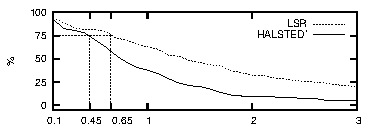
\includegraphics[width=3in]{lsrvscostpd.pdf}

% \% false alarms:

% 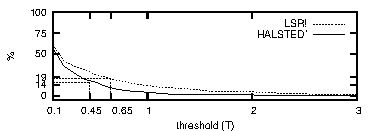
\includegraphics[width=3in]{lsrvscostpf.pdf}
% \end{center}}
% \caption{
%  Y-axis shows probability of false alarm,
%   and
%   probability of recognizing defective modules  seen using \mbox{$d_i \ge T$}.
%   Curves calculated from the KC2 dataset from the PROMISE repository goo.gl/pGDfvp.
%  }\label{fig:pd1}
%  \end{figure}
 
% Note that either the Halstead or LOC detector can reach some desired
% level of recall, regardless of their correlations, just by
% selecting the appropriate threshold value. For example, in \fig{pd1}, see the recall=75\% values
% found at {\em either} $d_i\ge 0.65$ or $d_2\ge 0.45$ (and at the threshold, the false alarm rates
% were very similar: 14\% and 19\%).

% The  point here is that   the true value of a detector
% could not be assessed {\em without} conducting a  tuning study in the context of some business case (in this case, 
% issuing a request to an inspection team to review some module).  
% Hence, it is important to explore tuning.

% The rest of this paper repeats the analysis of this section, but for 
% more complex learners.
 
%  \subsection{You Can't Always Get What You Want}\label{sect:goals}
 
%  Having made the case that tuning needs to be explored more,
%  but before we get into the technical details of this
%  paper, this section discusses some
%  general matters about setting goals during tuning
%  experiments.
 
%  This paper characterizes tuning as an optimization problem (how to change the settings on the learner
%  in order to best improve the output).
% With such optimizations,  it is not always possible to optimize for all goals at the same time.
% For example, the following text does not
% show results for tuning on recall
% or false alarms since optimizing {\em only} for those goals can lead
% to some undesirable side effects:
% \bi
% \item
% {\em Recall} reports the percentage of  predictions that are actual examples of  what we are looking for.
% When we tune for {\em recall}, we can achieve near
% 100\% recall-- but the cost of a near 100\% false alarms.
% \item
% {\em False alarms} is the percentage of other examples that are reported  (by the learner)
% to be part of the targeted examples.
% When we tune for {\em false alarms}, we 
% can achieve near zero percent false alarm rates by effectively turning off
% the detector (so the  recall falls to nearly zero).
% \ei
% Accordingly,  this paper  explores performance measures that comment on all 
% target classes: see the  precision and ``F'' measures discussed below: see {\em Optimization Goals}.
% That said, we are sometimes asked what good is a learner if it optimizers for (say) precision
% at the expense of (say) recall. 

% Our reply is that software engineering is a very diverse enterprise
% and that different kinds of development need to optimize for different goals
% (which may not necessarily be ``optimize for recall''):
% \bi
% \item
% Anda, Sjoberg and Mockus are concerned with {\em reproducibility}  and so
% assess their models using the the ``coefficient of variation'' $C\frac{stddev}{mean}$) ~\cite{anda09}.
% \item
% Arisholm~\&~Briand~\cite{arisholm06},  Ostrand \& Weyeuker~\cite{ostrand04} and Rahman et al.~\cite{rahman12} are concerned with reducing the work load associated with someone
% else reading a learned model, then applying it. Hence, they assess their models using  {\em reward}; i.e.   the fewest lines of code
%   containing the most bugs.
% \item
% Yin et al. are concerned about
%  {\em incorrect bug fixes}; i.e. those that require subsequent work in order to complete the bug fix.
% These bugs occur  when (say) developers try to fix parts of the code
% where they have very little experience~\cite{yin11}.  Hence, they assess a learned
% model using a measure that selects for  the most number of bugs in regions that {\em the most programmers have worked with before}.
% \item
% For safety critical applications, high false alarm rates are  acceptable if the cost
% of overlooking  critical issues outweighs the inconvenience of   inspecting a few more
% modules. 
% \item
% When rushing a product to market,  there is a business case to 
% avoid the extra rework associated with false alarms.  In that business context, 
% managers might be willing to lower the recall somewhat in order to minimize the false alarms.
% \item
% When the second author worked with contractors at  NASA's software independent verification
% and validation facility, he found  new contractors  
% only reported issues that were most certainly important defects; i.e. they minimized
%   false alarms even if that damaged their precision (since, they felt, 
% it was better to silent than wrong). Later on, once
% those contractors had acquired a reputation of being insightful members of the team,
% they improved their precision scores (even if it means some more false alarms).
% \ei
% Accordingly, this paper does not assume that (e.g.) minimizing false alarms is 
% more important than maximizing   precision or recall. Such a determination 
% depends on   business conditions.

% Rather, what we can  show  examples where  changing  optimization goals can also change 
% the conclusions made from that learner on that data. More generally, we caution that it is 
% important not to overstate  empirical results from  analytics.
% Those results need to be expressed {\em along with} the context within which they are
% relevant (and by ``context'', we mean the optimization goal).



\subsection{Tuning Algorithms}
In this section, we will discuss standard optimization problems and why choose DE as
a tuning algorithm in this paper.

In mathematics, computer science, mechanical engineering, and artificial intelligence,  most optimization
problems are to find the best solutions to maximize or minimize some objective given a defined domain.
Mathematically, optimization can be defined as following:

\begin{equation}\label{eq1}
  \begin{array}{ll}
    min  & f_0(X) \\
    s.t. & f_i(X) \leq b_i, i=1,...,m.
  \end{array}
\end{equation}

Here the vector $X = (x_1,...,x_n)$ is the parameter variables, and $f_0$ is the objective function,
and $f_i, i=1,...,m$ are the constraints function. The vector $X^*$ is the best solution if it has the 
smallest objective value among all vectors that satisfy the constraints\cite{boyd2004convex}.
Based on the properties of objective functions and constraints functions, like linearality or nonlinearity,
optimization problem can be classified into many different subfields. For example, if objective function
is convex (minimization) or concave (maximization) and the constraint function is convex, 
this optimization problem is {\em convex optimization}. This sort of problem 
could have a analytics solution by using corresponding algorithms, like {\em simplex algorithm}
can be used to solve {\em linear programming} problem. If the objecitve function or some of 
the constraints are nonlinear, then this problem is {\em nonlinear programming}.
Methods like {\em Newton's method and Gradient descent} are popular methods to solve such problems.
However, there exist another subfield where the real-world optimization problem is too complicated to
be described by analytical expressions and we have no prior knowledge about the problem being optimized, then
some heuristics, like {\em random search, genetic algorithms and simulated annealing},
are used to find approximate solutions for these sort of optimization problems.
% \end{array}
% A lot of optimization searching algorithms can be found in mathematical,
% evolutionary computation, and artificial intelligent fields.

\begin{algorithm}[!t]

\scriptsize
\begin{algorithmic}[1]
\Require $\mathit{np} = 10$, $f=0.75$, $cr=0.3$, $\mathit{life} = 5$, $\mathit{Goal} \in \{\mathit{pd},f,...\}$
\Ensure $S_{best}$
\vspace{2mm}
\Function{DE}{$\mathit{np}$, $f$, $cr$, $\mathit{life}$, $\mathit{Goal}$}
 \State $Population  \gets $ InitializePopulation($\mathit{np}$)   
 \State $S_{best} \gets $GetBestSolution($Population $)
 \While{$\mathit{life} > 0$}
\State $NewGeneration \gets \emptyset$
\For{$i=0 \to \mathit{np}-1$}
\State $S_i \gets$ Extrapolate($Population [i], Population , cr, f$)
\If {Score($S_i$) >Score($Population [i]$)}
\State $NewGeneration$.append($S_i$)
\Else
\State $NewGeneration$.append($Population [i]$)
\EndIf
\EndFor
\State $Population  \gets NewGeneration$
\If{$\neg$ Improve($Population $)}
\State $life -=1$
\EndIf
\State $S_{best} \gets$ GetBestSolution($Population $)
 \EndWhile
\State \Return $S_{best}$
\EndFunction
\Function{Score}{$Candidate$}
   \State set tuned parameters according to $Candidate$
   \State $model \gets$TrainLearner()
   \State $result \gets$TestLearner($model$)   
   \State \Return$\mathit{Goal}(result)$  
\EndFunction
\Function{Extrapolate}{$old, pop, cr, f$}
  \State $a, b, c\gets threeOthers(pop,old)$  
  \State $newf \gets \emptyset$
  \For{$i=0 \to \mathit{np}-1$}
       \If{$cr < random()$}
         \State $newf$.append($old[i]$)
                \Else
                  \If{typeof($old[i]$) == bool}
                    \State $newf$.append(not $old[i]$)
         \Else
          \State $newf$.append(trim($i$,($a[i] + f * (b[i] - c[i]$)))) 
         \EndIf
       \EndIf
  \EndFor
 \State \Return $newf$
\EndFunction
        \end{algorithmic} 
\caption{Pseudocode for DE with Early Termination}
\label{alg:DE}
\end{algorithm}
 


 \begin{table*}[t]

\renewcommand{\baselinestretch}{0.8}
\scriptsize
\centering
%   \begin{tabular}{p{0.75cm}p{0.75cm}p{0.75cm}p{0.75cm}p{0.75cm}p{0.75cm}p{0.75cm}p{0.75cm}p{0.75cm}p{0.75cm}}\hline
  \begin{tabular}{c c c c c c c c c c } \hline
  Dataset &antV0&antV1&antV2&camelV0&camelV1&ivy&jeditV0&jeditV1&jeditV2
\\\hline
  training &20/125 &40/178 &32/293 &13/339 &216/608 &63/111 &90/272 &75/306 &79/312
\\  tuning  &40/178 &32/293 &92/351 &216/608 &145/872 &16/241 &75/306 &79/312 &48/367
\\  testing &32/293 &92/351 &166/745 &145/872 &188/965 &40/352 &79/312 &48/367 &11/492
\\ \hline
  Dataset &log4j&lucene&poiV0&poiV1&synapse&velocity&xercesV0&xercesV1
\\\hline
  training &34/135 &91/195 &141/237 &37/314 &16/157 &147/196 &77/162 &71/440
\\  tuning  &37/109 &144/247 &37/314 &248/385 &60/222 &142/214 &71/440 &69/453
\\  testing &189/205 &203/340 &248/385 &281/442 &86/256 &78/229 &69/453 &437/588
\\  \end{tabular}

   \caption{Data used in this experiment. 
   E.g., the top left data set has 20 defective classes out of 125 total.
   See \tion{dataa} for explanation of {\em training, tuning, testing} sets.
   }\label{tab:data1}
\end{table*} 


Since there are so many optimization algorithms, how should researchers
select which optimizers to apply to tune data miners working 
with software engineering data? Predictive models, like defect predictor,
in software engineering have several limitations: the models are usually not
numerically differentiated; whether the response surfaces are smooth or non-smooth are unknown;
for some models, they have more parameters to tune, which will lead to a very complicated searching space. Due to these limitations, the most efficient searching algorithm
are likely to work well with software predictive models. Specifically,
{\em gradient} methods that are widely used in machine learning\cite{bengio2000gradient,maclaurin2015gradient} for 
hyper-parameters optimization are not suited to this situation because we could not have an analytical expression
to describe the objective function in terms of those parameters to be tuned and therefore gradients are usually unavailable; 
{\em Grid search} is a potentially expensive method as we show before\cite{tantithamthavorn2016automated} and suffers from ``curse of dimensionality''.
{\em tabu-search} struggles with
the high-dimensional optimization problem \cite{mayer1998tabu}; {\em Simulated annealing} 
has been considered a good tool for complex nonlinear optimization problems\cite{fea02a,me07f}, but one of the major drawbacks of the technique is its very slow convergence, especially for large searching space\cite{ram1996parallel}. Then the evolutionary algorithms will be
the most practical candidate tools.

There are various evolutionary algorihtms, like {\em genetic algorithms}\cite{goldberg79}, {\em differential evolution}~\cite{storn1997differential} and 
{\em particle swarm optimization}~\cite{pan08}.
Of these,   
differential evolution (DE) is the simplest one, which can be coded in less than a page of some high-level scripting language. Our reading of the current literature is that there are more  advocates for
differential evolution than
  the others as a optimization tool. For example,  Vesterstrom and Thomsen~\cite{Vesterstrom04} found DE to be competitive with 
  particle swarm optimization and other GAs. 
   
DEs have been applied before for   parameter tuning (e.g. see~\cite{omran2005differential, chiha2012tuning}) but this is the first time they have been applied to
optimize defect prediction from static code attributes.  
The pseudo-code for differential evolution is shown in Algorithm~\ref{alg:DE}.
In the following description, 
    superscript numbers denote lines in that pseudo-code.



%  \begin{table*}[!t]

% \renewcommand{\baselinestretch}{0.8}
% \scriptsize
% \centering
%   \begin{tabular}{c c c c c c c c c c }\hline
%   Dataset &antV0&antV1&antV2&camelV0&camelV1&ivy&jeditV0&jeditV1&jeditV2
% \\\hline
%   training &20/125 &40/178 &32/293 &13/339 &216/608 &63/111 &90/272 &75/306 &79/312
% \\  tuning  &40/178 &32/293 &92/351 &216/608 &145/872 &16/241 &75/306 &79/312 &48/367
% \\  testing &32/293 &92/351 &166/745 &145/872 &188/965 &40/352 &79/312 &48/367 &11/492
% \\ \hline
%   Dataset &log4j&lucene&poiV0&poiV1&synapse&velocity&xercesV0&xercesV1
% \\\hline
%   training &34/135 &91/195 &141/237 &37/314 &16/157 &147/196 &77/162 &71/440
% \\  tuning  &37/109 &144/247 &37/314 &248/385 &60/222 &142/214 &71/440 &69/453
% \\  testing &189/205 &203/340 &248/385 &281/442 &86/256 &78/229 &69/453 &437/588
% \\  \end{tabular}

%   \caption{Data used in this experiment. 
%   E.g., the top left data set has 20 defective classes out of 125 total.
%   See \tion{dataa} for explanation of {\em training, tuning, testing} sets.
%   }\label{tab:data1}
% \end{table*} 




DE evolves a {\em NewGeneration} of candidates  from
a current {\em Population}.  Our DE's lose one ``life''
when the new population is no better than  current one (terminating when ``life'' is zero)$^{L4}$.
Each candidate solution in the {\em Population}  
is a pair of {\em (Tunings, Scores)}.  {\em Tunings} are selected from
\tab{parameters} and {\em Scores} come from training a learner using those parameters
and applying it     test data$^{L23-L27}$.

The premise of DE  is that the best way to mutate the existing tunings
is to {\em Extrapolate}$^{L28}$
between current solutions.  Three solutions $a,b,c$ are selected at random.
For each tuning parameter $i$, at some probability {\em cr}, we replace
the old tuning $x_i$ with $y_i$. For booleans, we use $y_i= \neg x_i$ (see line 36). For numerics, $y_i = a_i+f \times (b_i - c_i)$   where $f$ is a parameter
controlling  cross-over.  The {\em trim} function$^{L38}$ limits the new
value to the legal range min..max of that parameter.
 
The main loop of DE$^{L6}$ runs over the {\em Population}, replacing old items
with new {\em Candidate}s (if  new candidate is better).
This means that, as the loop progresses, the {\em Population} is full of increasingly
more valuable solutions. This, in turn, also improves  the candidates, which are {\em Extrapolate}d
from the {\em Population}.

For the experiments of this paper, we collect performance
values from a data mining, from which a {\em Goal} function extracts one 
performance value$^{L26}$ (so we run this code many times, each time with
a different {\em Goal}$^{L1}$).  Technically, this makes a  {\em single objective} DE (and for notes on multi-objective DEs, see~\cite{Coello05,zhang07,5583335}).


%\begin{algorithm}
%\begin{algorithmic}[1]
% \KwData{this text}
% \KwResult{how to write algorithm with \LaTeX2e }
% initialization\;
% \While{not at end of this document}{
%  read current\;
%  \eIf{understand}{
%   go to next section\;
%   current section becomes this one\;
%   }{
%   go back to the beginning of current section\;
%  }
% }
% \caption{How to write algorithms}
% \end{algorithmic}
%\end{algorithm}